\section{Hacking Windows clock}

Sometimes I did some kind of first April prank for my coworkers.

Let's find, if we could do something with Windows clock?
Can we force to go clock hands backwards?

First of all, when you click on date/time in status bar, a \IT{C:\textbackslash{}WINDOWS\textbackslash{}SYSTEM32\textbackslash{}TIMEDATE.CPL} is running,
which is usual executable PE file.

Let's see, how it draw hands?
When I open the file (from Windows 7) in Resource Hacker, there are clock faces, but with no hands:

\begin{figure}[H]
\centering
\myincludegraphics{examples/timedate/reshack.png}
\caption{Resource Hacker}
\end{figure}

OK, what we know? How to draw a clock hand? All they are started at the middle of circle, ending with its border.
Hence, we need to calculate coordinates of a point on circle's border.
From school-level mathematics we may remember that we need to use sine/cosine functions to draw circle, or at least
square root.
There are no such things in \IT{TIMEDATE.CPL}, at least at first glance.
But, thanks to Microsoft debugging PDB files, I can find a function named \IT{CAnalogClock::DrawHand()}, which calls
\IT{Gdiplus::Graphics::DrawLine()} at least twice.

Here is its code:

\lstinputlisting{examples/timedate/1.lst}

\myindex{Windows!Win32!MulDiv()}
We can see that \IT{DrawLine()} arguments are dependent on result of \IT{MulDiv()} function
and a \IT{table[]} table (name is mine),
which has 8-byte elements (look at \INS{LEA}'s second operand).

What is inside of table[]?

\lstinputlisting{examples/timedate/2.lst}

It's referenced only from \IT{DrawHand()} function at has 120 32-bit words or 60 32-bit pairs... wait, 60?
Let's take a closer look at these values.
First of all, I'll zap 6 pairs or 12 32-bit words with zeroes, and then I'll put patched \IT{TIMEDATE.CPL}
into \IT{C:\textbackslash{}WINDOWS\textbackslash{}SYSTEM32}.
(You may need to set owner of the *TIMEDATE.CPL* file to your primary user account (instead of \IT{TrustedInstaller}),
and also, boot in safe mode with command prompt so you can copy the file, which is usually locked.)

\begin{figure}[H]
\centering
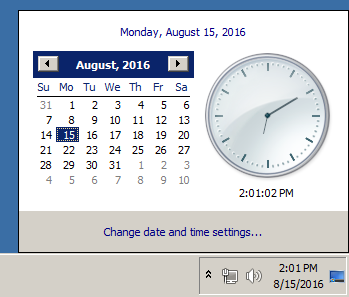
\includegraphics[width=0.5\textwidth]{examples/timedate/6_pairs_zeroed.png}
\caption{Attempt to run}
\end{figure}

Now when any hand is located at 0-5 seconds/minutes, it's invisible! However, opposite (shorter) part of second hand
is visible and moving.
When any hand is outside of this area, hand is visible as usual.

\myindex{Mathematica}
Let's take even closer look at the table in Mathematica.
I have copypasted table from the \IT{TIMEDATE.CPL} to a \IT{tbl} file (480 bytes).
We will take for granted the fact that these are signed values, because half of elements are below zero (0FFFFE0C1h, etc).
If these values would be unsigned, they would be suspiciously huge.

\begin{lstlisting}
	In[]:= tbl = BinaryReadList["~/.../tbl", "Integer32"]

	Out[]= {0, -7999, 836, -7956, 1663, -7825, 2472, -7608, 3253, -7308, 3999, \
	-6928, 4702, -6472, 5353, -5945, 5945, -5353, 6472, -4702, 6928, \
	-4000, 7308, -3253, 7608, -2472, 7825, -1663, 7956, -836, 8000, 0, \
	7956, 836, 7825, 1663, 7608, 2472, 7308, 3253, 6928, 4000, 6472, \
	4702, 5945, 5353, 5353, 5945, 4702, 6472, 3999, 6928, 3253, 7308, \
	2472, 7608, 1663, 7825, 836, 7956, 0, 7999, -836, 7956, -1663, 7825, \
	-2472, 7608, -3253, 7308, -4000, 6928, -4702, 6472, -5353, 5945, \
	-5945, 5353, -6472, 4702, -6928, 3999, -7308, 3253, -7608, 2472, \
	-7825, 1663, -7956, 836, -7999, 0, -7956, -836, -7825, -1663, -7608, \
	-2472, -7308, -3253, -6928, -4000, -6472, -4702, -5945, -5353, -5353, \
	-5945, -4702, -6472, -3999, -6928, -3253, -7308, -2472, -7608, -1663, \
	-7825, -836, -7956}

	In[]:= Length[tbl]
	Out[]= 120
\end{lstlisting}

Let's treat two consecutive 32-bit values as pair:

\begin{lstlisting}
	In[]:= pairs = Partition[tbl, 2]
	Out[]= {{0, -7999}, {836, -7956}, {1663, -7825}, {2472, -7608}, \
	{3253, -7308}, {3999, -6928}, {4702, -6472}, {5353, -5945}, {5945, \
	-5353}, {6472, -4702}, {6928, -4000}, {7308, -3253}, {7608, -2472}, \
	{7825, -1663}, {7956, -836}, {8000, 0}, {7956, 836}, {7825, 
	1663}, {7608, 2472}, {7308, 3253}, {6928, 4000}, {6472, 
	4702}, {5945, 5353}, {5353, 5945}, {4702, 6472}, {3999, 
	6928}, {3253, 7308}, {2472, 7608}, {1663, 7825}, {836, 7956}, {0, 
	7999}, {-836, 7956}, {-1663, 7825}, {-2472, 7608}, {-3253, 
	7308}, {-4000, 6928}, {-4702, 6472}, {-5353, 5945}, {-5945, 
	5353}, {-6472, 4702}, {-6928, 3999}, {-7308, 3253}, {-7608, 
	2472}, {-7825, 1663}, {-7956, 836}, {-7999, 
	0}, {-7956, -836}, {-7825, -1663}, {-7608, -2472}, {-7308, -3253}, \
	{-6928, -4000}, {-6472, -4702}, {-5945, -5353}, {-5353, -5945}, \
	{-4702, -6472}, {-3999, -6928}, {-3253, -7308}, {-2472, -7608}, \
	{-1663, -7825}, {-836, -7956}}

	In[]:= Length[pairs]
	Out[]= 60
\end{lstlisting}

Let's try to treat each pair as X/Y coordinate and draw all 60 pairs, and also first 15 pairs:

\begin{figure}[H]
\centering
\myincludegraphics{examples/timedate/math.png}
\caption{Mathematica}
\end{figure}

Now this is something!
Each pair is just coordinate.
First 15 pairs are coordinates for $\frac{1}{4}$ of circle.

Perhaps, Microsoft developers precalculated all coordinates and put them into table.

Now I can understand why when I zapped 6 pairs, hands were invisible at that area: in fact, hands were drawed,
they just had zero length, because hand started at 0:0 coordinate and ended there.

\subsubsection{The prank (practical joke)}

Given all that, how would we force hands to go counterclockwise?
In fact, this is simple, we need just to rotate the table, so each hand, instead of drawing at place of first second,
would be drawing at place of 59th second.

I made the patcher a long time ago, at the very beginning of 2000s, for Windows 2000.
Hard to believe, it still works for Windows 7, perhaps, the table hasn't been changed since then!

Patcher source code: \url{https://github.com/dennis714/random_notes/blob/master/timedate/time_pt.c}.

Now I can see all hands goes backwards:

\begin{figure}[H]
\centering
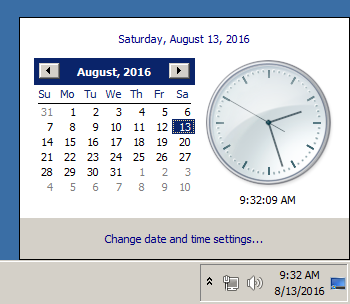
\includegraphics[width=0.5\textwidth]{examples/timedate/counterclockwise.png}
\caption{Now it works}
\end{figure}

Well, there is no animation in this article, but if you look closer, you can see, that hands are in fact shows correct
time, but the whole clock face is rotated vertically, like we see it from the inside of clock.

\subsubsection{Windows 2000 leaked source code}

So I did the patcher and then Windows 2000 source code has been leaked (I can't force you to trust me, though).
Let's take a look on source code if that function and table.
The file is \IT{win2k/private/shell/cpls/utc/clock.c}:

\begin{lstlisting}
	//
	//  Array containing the sine and cosine values for hand positions.
	//
	POINT rCircleTable[] =
	{
	    { 0,     -7999},
	    { 836,   -7956},
	    { 1663,  -7825},
	    { 2472,  -7608},
	    { 3253,  -7308},
	...
	    { -4702, -6472},
	    { -3999, -6928},
	    { -3253, -7308},
	    { -2472, -7608},
	    { -1663, -7825},
	    { -836 , -7956},
	};

	////////////////////////////////////////////////////////////////////////////
	//
	//  DrawHand
	//
	//  Draws the hands of the clock.
	//
	////////////////////////////////////////////////////////////////////////////

	void DrawHand(
	    HDC hDC,
	    int pos,
	    HPEN hPen,
	    int scale,
	    int patMode,
	    PCLOCKSTR np)
	{
	    LPPOINT lppt;
	    int radius;

	    MoveTo(hDC, np->clockCenter.x, np->clockCenter.y);
	    radius = MulDiv(np->clockRadius, scale, 100);
	    lppt = rCircleTable + pos;
	    SetROP2(hDC, patMode);
	    SelectObject(hDC, hPen);

	    LineTo( hDC,
	            np->clockCenter.x + MulDiv(lppt->x, radius, 8000),
	            np->clockCenter.y + MulDiv(lppt->y, radius, 8000) );
	}
\end{lstlisting}

Now it's clear: coordinates has been precalculated as if clock face has height and width of $2 \cdot 8000$,
and then it's rescaled to current clock face radius using \IT{MulDiv()} function.

POINT structure\footnote{\url{https://msdn.microsoft.com/en-us/library/windows/desktop/dd162805(v=vs.85).aspx}}
is a structure of two 32-bit values, first is \IT{x}, second is \IT{y}.

